\documentclass[aspectratio=169]{beamer}
\usetheme{metropolis}

%\usepackage{pgfpages}
%\setbeameroption{show notes}
%\setbeameroption{show notes on second screen=right}

\usepackage[english]{babel}
\usepackage[utf8]{inputenc}
\usepackage{amsmath, amssymb, amsthm, amsfonts}
\usepackage{multimedia}
\usepackage{graphics}
\usepackage{hyperref}

\usepackage{caption}
\usepackage{subcaption}

\title{Generelle Statistiske Metoder}
\author{Erik Rybakken}

\begin{document}

\frame{\titlepage}

\begin{frame}
  \frametitle{Framingham Datasett}
  \begin{itemize}
    \item Studie av 4434 pasienter, med fokus på hjerteproblemer.
    \pause
    \item Hver pasient ble undersøkt tre ganger, med 6 års mellomrom.
  \end{itemize}

  \pause

  To mulige problemstillinger:
  \begin{enumerate}
    \item Hvilke faktorer påvirker blodtrykket?
    \pause
    \item Kan vi forutsi hvor lenge en pasient har igjen å leve basert på dataene som ble gjort i første sjekk?
  \end{enumerate}
  Detaljer om analysen:
  \begin{enumerate}
    \item Kun pasientene fra den første sjekken ble brukt i analysen
    \pause
    \item Paientene med minst én ukjent verdi ble fjernet fra analysen
    \pause
    \item Dette ble i alt 3885 pasienter
  \end{enumerate}
\end{frame}

\begin{frame}
  \frametitle{Lineær regresjon}
  Vi antar en lineær modell:
  \begin{equation}
    Y = X \beta + \epsilon
  \end{equation}
  \pause
  der
  \begin{itemize}
    \item \(Y\) er responsen
    \item \(X\) er prediktorene
    \item \(\beta\) er en vektor med koeffisienter
    \item \(\epsilon\) er en normalfordelt variabel med forventningsverdi 0
  \end{itemize}
  \pause
  I vårt tilfelle er \(Y\) blodtrykket, mens \(X\) består av faktorene kjønn (mann/kvinne), alder,
  antall sigaretter røyket per dag, BMI, glukosenivå, utdanningsnivå og kolesterolnivå.
\end{frame}

\begin{frame}
  \frametitle{Minstre kvadraters metode}

  Vi har en \(n\times p\)-matrise \(\textbf{X}\) bestående av n observasjoner av p faktorer, og en \(n\times 1\)-matrise \(\textbf{Y}\) bestående av de korresponderene responsvariablene. Vi vil fra nå av anta at de observerte faktorene og responsene er normalisert til å ha gjennomsnitt 0 og varians 1.

  \pause

  Minstre kvadraters metode estimerer koeffisientene \(\beta\) ved å minimere RSS (residual sum of squares):

  \begin{equation}
    (\textbf{Y} - \textbf{X}\beta)(\textbf{Y} - \textbf{X}\beta)^T
  \end{equation}

  \pause
  Bruker alle faktorene, og kan føre til overfitting, og dermed dårligere prediksjon.
\end{frame}

\begin{frame}
  \frametitle{Tre forbedringer av minstre kvadraters metode}
  \begin{itemize}
    \item Beste delmengde-utvalg velger ut en delmengde av faktorene og utfører minstre kvadrater på denne.
    \pause
  \item Lasso-regresjon krymper absoluttverdien til koeffisientene \(\beta\).
    \pause
    \item Prinsipalkomponent-regresjon projiserer først faktorene til et lavere-dimensjonalt underrom og utfører deretter minstre kvadrater.
  \end{itemize}
\end{frame}

\begin{frame}
  \frametitle{Beste delmengde-utvalg}
  Gitt en delmengde \(S \subset \{1,\dots,p\}\) kan vi danne matrisen \(\textbf{X}_S = (\textbf{X}_{i_1}|\textbf{X}_{i_2}|\dots |\textbf{X}_{i_k})_{i_* \in S}\).
  Vi kan så utføre minst kvadrater på \(\textbf{X}_S\).
  \pause
  For en gitt \(0 \leq k \leq p\) utfører vi minste kvadrater på den delmengden \(S\) med \(|S| = k\) som gir lavest RSS.
\end{frame}

\begin{frame}
  \frametitle{Beste delmengde-utvalg}
  \begin{center}
    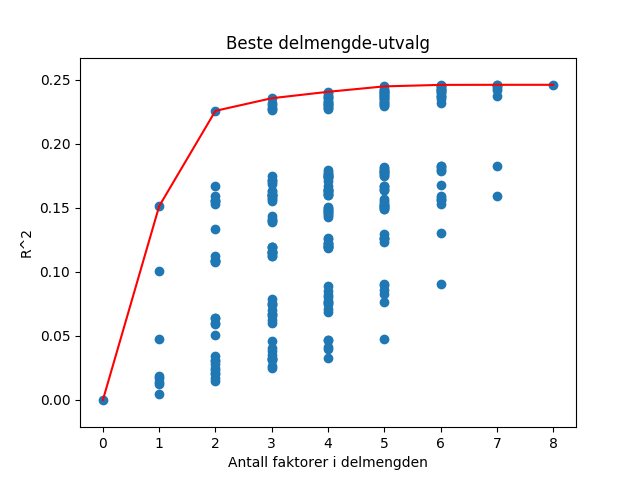
\includegraphics[height=0.8\textheight]{best_subset.png}
  \end{center}
\end{frame}

\begin{frame}
  \frametitle{Lasso-regresjon}
  Lasso-regresjon finner koeffisientene \(\beta\) som minimerer uttrykket
  \begin{equation}
    (\textbf{Y} - \textbf{X}\beta)(\textbf{Y} - \textbf{X}\beta)^T + \lambda \sum_{i=1}^p |\beta_i|
  \end{equation}
  der \(\lambda\) er en parameter som bestemmer hvor mye store koeffisienter skal straffes. Dette er ekvivalent med å minimere uttrykket
  \begin{equation}
    (\textbf{Y} - \textbf{X}\beta)(\textbf{Y} - \textbf{X}\beta)^T
  \end{equation}
  der vi krever at \(\sum_{i=1}^p |\beta_i| \leq t\).
\end{frame}

\begin{frame}
  \frametitle{Lasso-regresjon}
  \begin{center}
    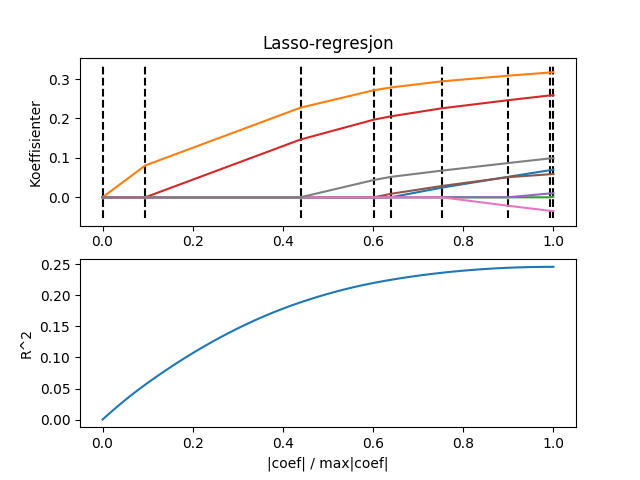
\includegraphics[height=0.8\textheight]{lasso.png}
  \end{center}
\end{frame}

\begin{frame}
  \frametitle{Prinsipalkomponent-regresjon}

  Matrisen \(\textbf{X}^T \textbf{X}\) kan dekomponeres (egenverdi-dekomposisjon):
  \begin{equation}
    \textbf{X}^T\textbf{X} = \textbf{VD}^2\textbf{V}^T
  \end{equation}

  der \(\textbf{V}\) er matrisen med egenvektorene til \(\textbf{X}^T\textbf{X}\) som kolonnevektorer og \(\textbf{D}^2\) er diagonalmatrisa med de korresponderende egenverdiene \(d_1^2 \geq d_2^2 \geq \dots \geq d_p^2\) som diagonalelementer.

  \pause

  Vi danner matrisa \(\textbf{Z} = \textbf{X}\textbf{V}\). Kolonnene i denne matrisa kalles \emph{prinsipalkomponentene} til \textbf{X}. Den \(n\)-te prinsipalkomponenten har maksimal varians gitt at den skal være ortogonal til de forrige \(n-1\) prinsipalkomponentene. 

\end{frame}

\begin{frame}
  \frametitle{Prinsipalkomponent-regresjon}

  Prinsipalkomponent-regresjon utføres ved at man velger de \(k\) første prinsipalkomponentene til \(X\), dvs. de første \(k\) kolonnene til \(Z\) og gjør minste kvadrater på denne matrisa.
\end{frame}

\begin{frame}
  \frametitle{Prinsipalkomponent-regresjon}
  \begin{center}
    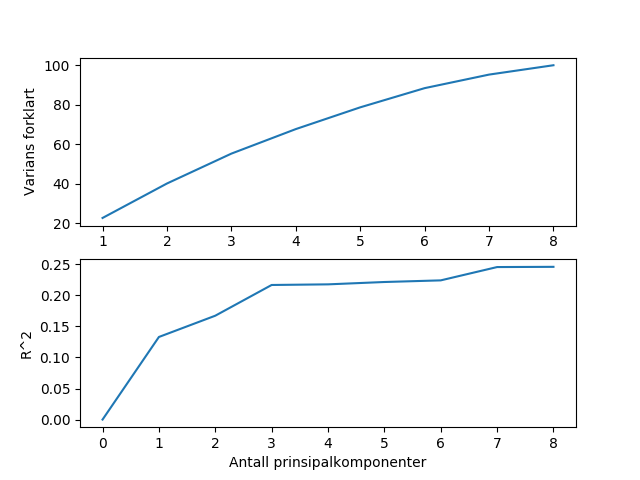
\includegraphics[height=0.8\textheight]{pcr.png}
  \end{center}
\end{frame}

\begin{frame}
  \frametitle{Parametervalg}
  Aller først delte jeg datasettet i to deler: Ett treningssett med 3108 (\(80\%\)) pasienter og et valideringssett med 777 (\(20\%\)) pasienter.
  \pause
  For å bestemme parameterene til de tre metodene, brukte jeg kryss-validering.
  \pause
  \begin{itemize}
    \pause
    \item Treningssettet ble delt inn i 10 grupper.
    \pause
    \item Hver modell og valg av parameter ble trent på 9 grupper og testet på den siste.
    \pause
    \item Dette ble gjentatt for hver gruppe.
    \pause
    \item Gjennomsnittet av RSS ble beregnet for hver gruppe.
    \pause
    \item Jeg valgte den parameteren med lavest gjennomsnittlig RSS.
  \end{itemize}
\end{frame}

\begin{frame}
  \frametitle{Beste delmengde-utvalg}
  \begin{center}
    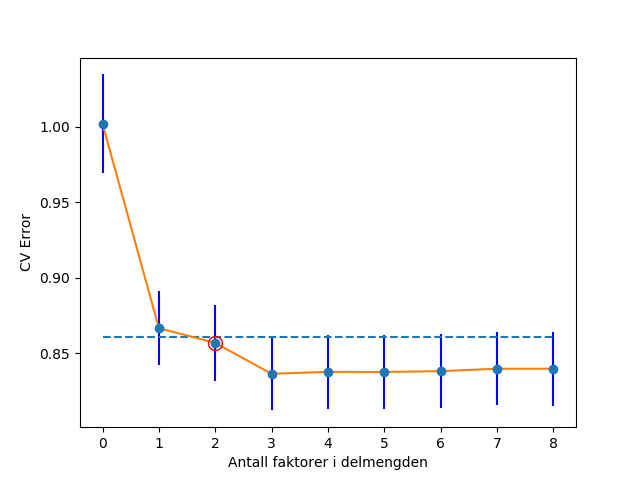
\includegraphics[height=0.8\textheight]{best_subset_CV.png}
  \end{center}
\end{frame}

\begin{frame}
  \frametitle{Lasso-regresjon}
  \begin{center}
    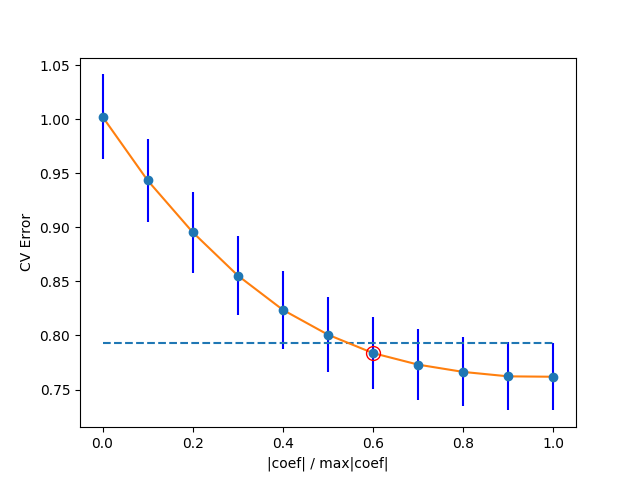
\includegraphics[height=0.8\textheight]{lasso_CV.png}
  \end{center}
\end{frame}

\begin{frame}
  \frametitle{Prinsipalkomponent-regresjon}
  \begin{center}
    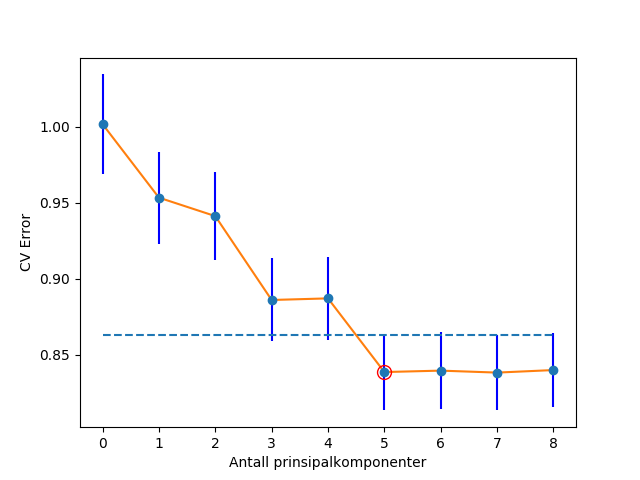
\includegraphics[height=0.8\textheight]{pcr_CV.png}
  \end{center}
\end{frame}

\begin{frame}
  \frametitle{Resultater}
  \begin{tabular}{ l r r r r}
    Faktor & Minste kvadrater & Beste delmengde & Lasso & PCR \\
    \hline
    Kjønn & 0.070 & 0.070 & 0.052 & 0.071 \\
    Alder & 0.317 & 0.323 & 0.309 & 0.317 \\
    Sigaretter per dag & 0.002 & & & 0.002 \\
    BMI & 0.259 & 0.264 & 0.259 & 0.246 \\
    Diabetiker & 0.010 & & 4.085 & 0.032 \\
    Glukose-nivå & 0.059 & 0.066 & 0.051 & 0.037 \\
    Utdanningsnivå & -0.034 & & -0.021 & -0.035 \\
    Kolesterol-nivå & 0.099 & 0.097 & 0.087 & 0.100 \\
    \hline
    Test Error & 0.723 & 0.721 & 0.720 & 0.723 \\
    Std Error & 0.039 & 0.039 & 0.039 & 0.039 \\
  \end{tabular}
\end{frame}

\begin{frame}
  \frametitle{Utvidelse av metodene}

  Jeg dannet nye faktorer ved å ta alle mulige produkter av de originale: \[X_1 \cdot X_1, X_1 \cdot X_2, \dots.\]
  \pause
  Disse faktorene ble brukt til å danne en ny matrise \(\textbf{X}\) bestående av både de originale og de nye faktorene, tilsammen 44 faktorer.
  \pause
  Jeg utførte så Lasso-regresjon og PCR på denne nye matrisen.
\end{frame}

\begin{frame}
  \frametitle{Lasso-regresjon (del 2)}
  \begin{center}
    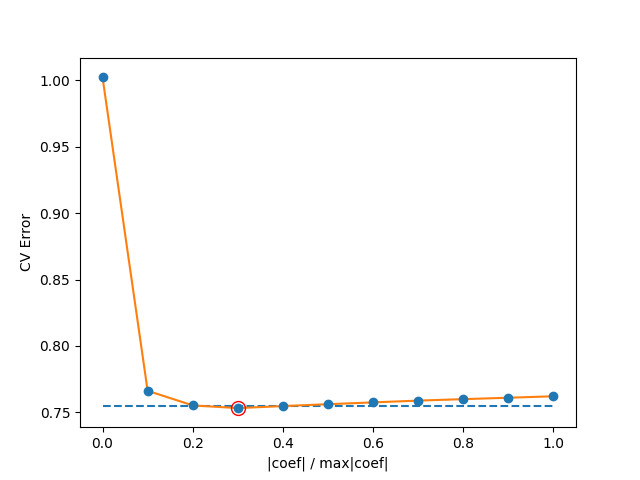
\includegraphics[height=0.8\textheight]{lasso_CV2.png}
  \end{center}
\end{frame}

\begin{frame}
    \frametitle{Prinsipalkomponent-regresjon (del 2)}
  \begin{center}
    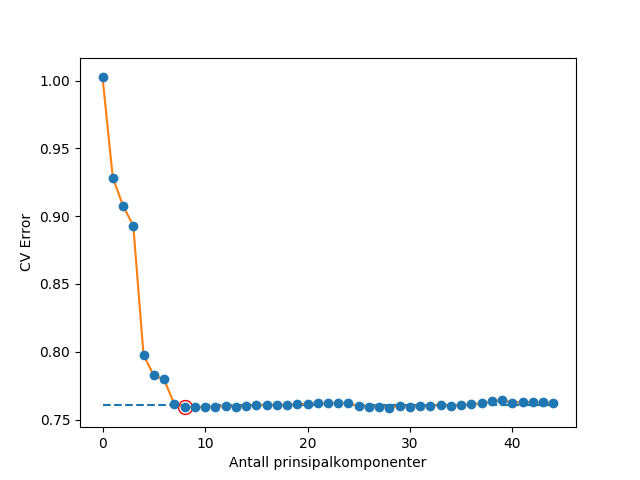
\includegraphics[height=0.8\textheight]{pcr_CV2.png}
  \end{center}
\end{frame}

\begin{frame}
  \frametitle{Resultater}
\begin{center}
  \begin{tabular}{ l r r}
     & Lasso & PCR \\
    \hline
    Test Error & 0.703 & 0.720 \\
    Std Error & 0.038 & 0.039
  \end{tabular}
  \end{center}

  Vi ser at Lasso-regresjon ble forbedret fra 0.720 til 0.703.
\end{frame}

\end{document}
